\section{Appendix}\label{App}
\noindent
In this section, we report an extension of the MINLP formulation presented in Section \ref{Form}, for dealing with the case of nonhomogeneous fleets of drones.
\noindent
In the following, we introduce the parameters or input data that formally describe the problem and that are summarized in Table \ref{table:At1}.
\noindent
\JP{The formulation in this appendix is rather similar to the one in Section \ref{subsec:CO} but, because of the assumption of nonhomogeneous drones, it needs to keep track of the drones used in each action. This implies to include an extra index $\delta$ in most of the variables. For the sake of completeness, we have included the complete set of constraints of this formulations although some of them are similar to those in Section \ref{subsec:CO}. Table \ref{table:At2} summarizes all the decision variables used in this formulation.}

\begin{table}[!h]
\scriptsize
\centering
%\color{blue}
\begin{tabular}{ | l | }
\hline
\textbf{Problem Parameters}\\
\hline
$origin$: coordinates of the point defining the origin of the mothership path (or tour).\\
$dest$: coordinates of the point defining the destination of the mothership path (or tour).\\
$\mathcal{G}$: set of the target graphs.\\
$g = (V_g, E_g)$: set of nodes and edges of each target graph $g \in \mathcal{G}$.\\
$\mathcal{L}(e_g)$: length of edge $e$ of graph $g \in \mathcal{G}$.\\
$\mathcal{L}(g)=\sum_{e_g\in E_g} \mathcal L(e_g)$: total length of the graph $g\in\mathcal G$.\\
$B^{e_g}, C^{e_g}$: coordinates of the endpoints of edge $e$ of graph $g \in \mathcal{G}$.\\
$\alpha^{e_g}$: fraction of edge $e$ of graph $g \in \mathcal{G}$ that must be visited.\\
$\alpha^{g}$: fraction of graph $g \in \mathcal{G}$ that must be visited.\\
$v_M$: mothership speed.\\
$\mathcal D$: set of drones.\\
$v_\delta$: drone $\delta$ speed.\\
$N_\delta$: drone $\delta$ endurance. \\
$\mathcal{O}$: set of drones operations to perform visits to the target graphs\\
$M$: big-M constant.\\
\hline
\end{tabular}
\caption{Nomenclature for AMMDRPG with non-homogeneous fleet of drones}
\label{table:At1}
\end{table}

\begin{table}[h!]
%\tiny
\scriptsize
\centering
%\color{blue}
\begin{tabular}{|l|}
\hline 
\textbf{Binary and Integer Decision Variables}\\
\hline
$\mu^{e_g} \in \{0,1\}, \:\: \forall e_g \in E_g\:\: (g \in \mathcal{G})$: equal to 1 if edge $e$ of graph $g$ (or a fraction of it) is visited by the drone, 0 otherwise.\\
$\text{entry}^{e_g} \in \{0,1\}, \:\: \forall e_g \in E_g\:\: (g \in \mathcal{G})$: auxiliary binary variable used for linearizing expressions.\\
$u^{e_{g}o\delta} \in \{0,1\}, \:\: \forall e_g \in E_g\:\: (g \in \mathcal{G}), \:\:\forall o \in \mathcal O, \:\: \forall \delta \in \mathcal D$: equal to 1 if the drone $\delta$ enters in graph $g$ by the edge $e_g$ at operation $o$,\\ \hspace*{1cm} 0 otherwise.\\
$z^{e_{g}e^{'}_{g}} \in \{0,1\}, \:\: \forall e_g, e_g' \in E_g\:\: (g \in \mathcal{G})$: equal to 1 if the drone goes from $e_g$ to $e^{'}_{g}$, 0 otherwise.\\
$v^{e_{g}o\delta} \in \{0,1\}, \:\: \forall e_g \in E_g\:\: (g \in \mathcal{G}), \:\: \forall o \in \mathcal O, \:\: \forall \delta \in \mathcal D$: equal to 1 if the drone $\delta$ exits from graph $g$ by $e_g$ at operation $o$,\\ \hspace*{1cm} 0 otherwise.\\
\hline
\textbf{Continuous Decision Variables}\\
\hline
$s^{e_g}\in[0, |E_g|-1],\:\: \forall e_g \in E_g\:\: (g \in \mathcal{G})$: continuous non negative variable representing the order of visit of the edge $e$ of graph $g$.\\
$\rho^{e_g} \in [0,1]$ and $\lambda^{e_g} \in [0,1], \:\: \forall e_g \in E_g\:\: (g \in \mathcal{G})$: defining the entry and exit points on $e_g$.\\
$\nu_\text{min}^{e_g}$ and $\nu_\text{max}^{e_g} \in [0,1], \:\: \forall e_g \in E_g\:\: (g \in \mathcal{G})$: auxiliary variables used for linearizing expressions.\\
$p^{e_g}\in [0, 1], \:\: \forall e_g \in E_g\:\: (g \in \mathcal G)$: auxiliary variable used for modelling the product of $\mu^{e_g}$ and $|\lambda^{e_g}-\rho^{e_g}|$.\\
$x_L^o\in\mathbb R^2, \:\: \forall o \in \mathcal O$: coordinates representing the point where the mothership launches the drones at operation $o$.\\
$x_R^o\in\mathbb R^2, \:\: \forall o \in \mathcal O$: coordinates representing the point where the mothership retrieves the drones at operation $o$.\\
$R^{e_g}\in\mathbb R^2, \:\: \forall e_g \in E_g\:\: (g \in \mathcal{G})$: coordinates representing the entry point on edge $e_g$ of graph $g$.\\
$L^{e_g}\in\mathbb R^2, \:\: \forall e_g \in E_g\:\: (g \in \mathcal{G})$: coordinates representing the exit point on edge $e_g$ of graph $g$.\\
$d_L^{e_go\delta} \geq 0, \:\: \forall e_g \in E_g\:\: (g \in \mathcal{G}),\:\: \forall o \in \mathcal O, \:\: \forall \delta\in\mathcal D$: representing the distance travelled by the drone $\delta$ from the launching\\
\hspace*{1cm} point $x_L^o$ on the mothership at operation $o$ to the first visiting point $R^{e_g}$ on $e_g$.\\
$p_L^{e_go\delta} \geq 0, \:\: \forall e_g \in E_g\:\: (g \in \mathcal{G}), \:\:\forall o \in \mathcal O, \:\:\forall \delta\in\mathcal D$: auxiliary variable used for modelling the product of $d_L^{e_go\delta}$ and $u^{e_go\delta}$.\\
$d^{e_g} \geq 0, \:\: \forall e_g \in E_g \:\: (g \in \mathcal{G})$: representing the distance travelled by the drone from the rendezvous point $R^{e_g}$ to the \\
\hspace*{1cm} launching point $L^{e_g}$ on $e_g$. \\
$d^{e_ge^\prime_g} \geq 0, \:\: \forall e_g, e^\prime_g \in E_g \:\: (g \in \mathcal{G})$: representing the distance travelled by the drone from the launching point $L^{e_g}$ on $e_g$ to\\
\hspace*{1cm}  the rendezvous point $R^{e^\prime_g}$ on $e^\prime_g$.\\
$p^{e_ge^\prime_g} \geq 0, \:\: \forall e_g, e^\prime_g \in E_g \:\: (g \in \mathcal{G})$: auxiliary variable used for modelling the product of $d^{e_ge^\prime_g}$ and $z^{e_ge^\prime_g}$.\\
$d_R^{e_go\delta} \geq 0, \:\: \forall e_g \in E_g\:\: (g \in \mathcal{G}), \:\: \forall o \in \mathcal O, \:\:\forall \delta\in\mathcal D$: representing the distance travelled by the drone $\delta$ from the last visiting point\\
\hspace*{1cm} $L^{e_g}$ on $e_g$ to the rendezvous point $x_R^o$ on the mothership at operation $o$.\\
$p_R^{e_go\delta} \geq 0, \:\: \forall e_g \in E_g\:\: (g \in \mathcal{G}), \:\:\forall o \in \mathcal O, \:\:\forall \delta\in\mathcal D$: auxiliary variable used for modelling the product of $d_R^{e_go\delta}$ and $v^{e_go\delta}$.\\
$d_{origin}\geq 0$: distance from the origin $origin$ to the first launching point $x_L^1$.\\
$d_{LR}^o \geq 0, \:\: \forall o \in \mathcal O$: representing the distance travelled by the mothership from the launching point $x_L^o$ to the rendezvous\\
\hspace*{1cm}   point $x_R^o$ at operation $o$.\\
$d_{RL}^o \geq 0, \:\: \forall o \in \mathcal O\setminus|\mathcal O|$: representing the distance travelled by the mothership from the rendezvous point $x_R^o$ at operation $o$ to the \\ 
\hspace*{1cm}  launching point $x_L^{(o+1)}$ at operation $o+1$.\\
$d_{dest}\geq 0$: distance from the last retrieving point $x_R^{|\mathcal O|}$ to the destination $dest$.\\
$time_D^o \geq 0, \:\: \forall o \in \mathcal O$: maximum time spent by a drone during operation $o$.\\
$time_M^o \geq 0, \:\: \forall o \in \mathcal O$: time spent by the mothership to go from the launching point $x_L^o$ to the retrieving point $x_R^o$ of operation $o$.\\
$time_M \geq 0$: total time spent by the mothership to go from the origin to the destination.\\
\hline
\end{tabular}
\caption{Decision Variables for AMMDRPG with non-homogeneous fleet of drones}
\label{table:At2}
\end{table}

\subsection*{Visits of graphs}
\noindent
As for the case of a homogeneous fleet of drones presented in Section \ref{Form}, to represent the movement of the drone within a graph $g\in\mathcal G$, we proceed to introduce some notation related to $g$.
Let $g = (V_g, E_g)$ be a graph in $\mathcal G$ whose total length is denoted by $\mathcal L(g)$. Here, $V_g$ denotes the set of nodes and $E_g$ denotes the set of edges connecting pairs of nodes.  Let $e_g$ be the edge $e$ of the graph $g \in G$ and let $\mathcal  L(e_g)$ be its length. Each edge $e_g$ is parameterized by its endpoints $B^{e_g}= (B^{e_g}(x_1), B^{e_g}(x_2))$ and $C^{e_g}= (C^{e_g}(x_1), C^{e_g}(x_2))$ and we can compute its length $\mathcal L(e_g) =\|C^{e_g} -  B^{e_g}\|$. 
\noindent
For each edge $e_g$ it is associated an indicator binary variable $\mu^{e_g}$ that is one if the drone visits the segment $e_g$. Moreover, we define the entry and exit points $R^{e_g}=(B^{e_g},C^{e_g},\rho^{e_g})$ and $L^{e_g}=(B^{e_g},C^{e_g},\lambda^{e_g})$ that determine the fraction of the edge visited by the drone. The coordinates of the points $R^{e_g}$ and $L^{e_g}$ are given, respectively by 
$$R^{e_g} = \rho^{e_g} B^{e_g} + (1- \rho^{e_g})C^{e_g} \quad\text{ and }\quad L^{e_g} = \lambda^{e_g} B^{e_g} + (1- \lambda^{e_g})C^{e_g},$$ where $\rho^{e_g} \in [0,1]$ and $\lambda^{e_g} \in [0,1]$ are variables to determine the position of the points on the segment.

\noindent
As discussed in Section \ref{section:desc}, we consider two modes of visit to the target graphs $g\in \mathcal{G}$:
\begin{itemize}
    \item Visiting a fraction $\alpha^{e_g}$ of each edge $e_g$ which can be modeled by using the following constraints:
    \begin{equation}\label{eq:NOalphaE}\tag{$\alpha$-E}
    |\lambda^{e_g} - \rho^{e_g}|\geq \alpha^{e_g}, \quad \forall e_g\in E_g.
    \end{equation}
    These inequalities state that the difference between the parametrizations of the entry and exit points associated to each edge $e_g$ must be higher than the fraction of the length of $e_g$ required to be traversed.
    \item Visiting a fraction $\alpha^g$ of the total length of the graph:
    \begin{equation}\label{eq:NOalphaG}\tag{$\alpha$-G}
    \sum_{e_g\in E_g} \mu^{e_g}|\lambda^{e_g} - \rho^{e_g}|\mathcal L(e_g) \geq \alpha^g\mathcal L(g).
    \end{equation}
    \noindent
    This constraint ensures that the sum of the fractions of the length of those edges chosen to be crossed must be higher than the fraction of the length of $g$ required to be traversed.
\end{itemize}



\bigskip
\noindent
In both cases, the corresponding constraints are nonlinear. To linearize them, we need to introduce a binary variable $\text{entry}^{e_g}$ that determines the traveling direction on the edge $e_g$ as well as the definition of the auxiliary variables $\nu_\text{min}^{e_g}$ and $\nu_\text{max}^{e_g}$ of the access and exit points on that segment. Then, for each edge $e_g$, the absolute value constraint \eqref{eq:NOalphaE} can be represented by:


\begin{equation}\label{eq:NOalpha-E}\tag{$\alpha$-E}
 |\rho^{e_g}-\lambda^{e_g}|\geq \alpha^{e_g} \Longleftrightarrow
 \left\{
 \begin{array}{ccl}
  \rho^{e_g} - \lambda^{e_g}                       & =    & \nu_\text{max}^{e_g} - \nu_\text{min}^{e_g},                                     \\
  \nu_\text{max}^{e_g}                         & \leq & 1-{\text{entry}^{e_g}},                                   \\
  \nu_\text{min}^{e_g}                      & \leq & {  \text{entry}^{e_g}},                                        \\
    \nu_\text{min}^{e_g}, \,\nu_\text{max}^{e_g} & \geq & 0, \\

  \nu_\text{max}^{e_g} + \nu_\text{min}^{e_g} & \geq & \alpha^{e_g}.
  \\
 \end{array}
 \right.
\end{equation}

\noindent
The first four inequalities model the standard trick of the linearization of the absolute value. The last constraint ensures that the value of the linear expression of the absolute value is higher than the required fraction $\alpha^{e_g}$.
\noindent
Similarly, \eqref{eq:NOalphaG} can be linearized as follows:
\begin{equation}\label{eq:NOalpha-G}\tag{$\alpha$-G}
 \sum_{e_g\in E_g} \mu^{e_g}|\rho^{e_g}-\lambda^{e_g}|\mathcal L(e_g)\geq \alpha^g\mathcal L(g). \Longleftrightarrow
 \left\{
 \begin{array}{ccl}
  \rho^{e_g} - \lambda^{e_g}                       & =    & \nu_\text{max}^{e_g} - \nu_\text{min}^{e_g},                                     \\
  \nu_\text{max}^{e_g}                         & \leq & 1-{\text{entry}^{e_g}},                                   \\
  \nu_\text{min}^{e_g}                      & \leq & {  \text{entry}^{e_g}},                                        \\
  \nu_\text{min}^{e_g}, \,\nu_\text{max}^{e_g} & \geq & 0, \\
  p^{e_g} & \leq & \nu_\text{max}^{e_g} + \nu_\text{min}^{e_g}, \\
  p^{e_g} & \leq & \mu^{e_g}, \\
  p^{e_g} & \geq & \nu_\text{max}^{e_g} + \nu_\text{min}^{e_g} + \mu^{e_g} - 1, \\
  \sum_{e_g\in E_g} p^{e_g}\mathcal L(e_g) & \geq & \alpha^{g}\mathcal L(g),
  \\
 \end{array}
 \right.
\end{equation}
where $p^{e_g}$ is the auxiliary variable that represents the product of the binary variable $\mu^{e_g}$ and the absolute value difference $|\rho^{e_g} - \lambda^{e_g}|$. The first four inequalities linearize again the absolute value expression. The (second) following three constraints model the product of the expression of the absolute value and the binary variable $\mu^{e_g}$. The last inequality ensures that the fraction of the length of those edges chosen to be crossed must be higher than the fraction of the length of $g$ required to be traversed.

\subsection*{Elimination of subtours}
\noindent
As already presented in Section \ref{Form},  to prevent the existence of subtours within each graph $g\in \mathcal G$ that the drone must visit, one can include, among others, either the compact formulation that uses the Miller-Tucker-Zemlin constraints (MTZ) or the subtour elimination constraints (SEC).\\
\noindent
For the MTZ formulation, we use the continuous variables $s^{e_g}$, defined in Table \ref{table:At2}, that state the order to visit the edge $e_g$ and set the following constraints for each $g\in\mathcal G$:

\begin{align}
    s^{e_g} - s^{e^\prime_g} + |E_g|z^{e_ge^\prime_g} & \leq |E_g| - 1  , &\quad\forall e_g \neq e_g'\in E_g, \tag{MTZ$_1$} \label{NOMTZ1}\\
    0 & \leq s^{e_g} \leq |E_g| - 1, &\quad\forall e_g\in E_g.\tag{MTZ$_2$}\label{NOMTZ2}
\end{align}

\noindent
Alternatively, we can also use the family of subtour elimination constraints for each $g\in\mathcal G$:
\begin{equation}\tag{SEC}\label{NOSEC}
    \sum_{e_g, e^\prime_g \in S} z_g^{e_ge^\prime_g} \leq |S| - 1, \quad \forall S\subset E_g.
\end{equation}

\noindent
To find SEC inequalities, as usual, we search for disconnected components in the current solution. Among them, we choose the shortest subtour found in the solution to be added as a lazy constraint to the model.\\

\subsection*{Drone constraints}
\noindent
To model this problem, as already described in Section \ref{subsec:CO}, we adopt the concept of operation.
%we use operations identified with the order in which the different target graphs in the problem are visited.
Let us denote by $\mathcal O$ the set of operations that the mothership and the fleet of drones have to carry out. These operations are visits to the different graphs in $\mathcal G$ with the required constraints. An operation $o\in\mathcal O$ is referred to as the event in which the mothership launches some drones from a taking-off location, denoted by $x_L^o$ and later it takes them back on a rendezvous location $x_R^o$. 
%Here, it is important to realize that both locations $x_L^o$ and $x_R^o$ must be determined in the continuous space where the mothership is assumed to move. Note that $|\mathcal O|\leq|\mathcal G|$, since it is assumed that, for each operation, at least one drone must be launched.
\noindent
For each operation $o\in\mathcal O$, each one of the drones launched from the mothership must follow a path starting from and returning to the mothership, while visiting the required edges of $g$.

%According to the notation introduced above, we write this generic path in the following form:


%$$
%x_L^o\rightarrow R^{e_g}\rightarrow L^{e_g}\rightarrow\ldots\rightarrow R^{e^\prime_g}\rightarrow L^{e^\prime_g}\rightarrow \ldots \rightarrow R^{e''_g} \rightarrow L^{e''_g} \rightarrow x_R^o.
%$$



\noindent
To include the definition of these paths in our mathematical programming formulation, we need to make decisions to choose:
\begin{itemize}
    \item The optimal assignment of drones for visiting graphs in a given operation $o$.
    \item The order to visit the edges of each graph in its corresponding operation.
\end{itemize}

\noindent
We model the route that the drone follows by using the binary variables $u^{e_go\delta}$, $z^{e_ge^\prime_g}$ and $v^{e_go\delta}$ defined in Table \ref{table:At2}.

\begin{align}
    \sum_{g\in \mathcal G}\sum_{e_g\in E_g}  u^{e_go\delta} & \leq 1, &\forall o\in \mathcal O, \forall \delta\in\mathcal D.\label{st:NODEnt}\\
    \sum_{g\in \mathcal G}\sum_{e_g\in E_g}  v^{e_go\delta} & \leq 1, &\forall o\in \mathcal O, \forall \delta\in\mathcal D.\label{st:NODExt} \\
    \sum_{e_g\in E_g} \sum_{o\in \mathcal O} \sum_{\delta\in\mathcal D} u^{e_go\delta} & = 1, &\forall g\in\mathcal G, \label{st:NODEng}\\%\tag{D
    \sum_{e_g\in E_g} \sum_{o\in \mathcal O} \sum_{\delta\in\mathcal D} v^{e_go\delta} & = 1, &\forall g\in\mathcal G, \label{st:NODExg}\\%\tag{D
    \sum_{e_g\in E_g} u^{e_go\delta} & = \sum_{e_g\in E_g} v^{e_go\delta}, &\forall g\in\mathcal G, \forall o\in \mathcal O, \forall \delta\in\mathcal D, \label{st:NODuv}\\%\tag{D
     \sum_{o\in \mathcal O} \sum_{\delta \in \mathcal D} u^{e_go\delta} + \sum_{e^\prime_g\in E_g} z_g^{e^\prime_ge_g} & = \mu^{e_g}, &\forall e_g\in E_g:g\in\mathcal G, \label{st:NODInu}\\
     \sum_{o\in \mathcal O} \sum_{\delta \in \mathcal D} v^{e_go\delta} + \sum_{e^\prime_g\in E_g} z_g^{e_ge^\prime_g} & = \mu^{e_g}, &\forall e_g\in E_g:g\in\mathcal G. \label{st:NODInv}
\end{align}

\noindent 
 Inequalities \eqref{st:NODEnt} and \eqref{st:NODExt} state that a drone $\delta$ visits at most one graph $g$ at operation $o$.  Constraints \eqref{st:NODEng} and \eqref{st:NODExg} assure that each graph is visited at some operation $o$ by some drone $\delta$. Equations \eqref{st:NODuv} ensure that the operation of entering and exiting from the graph $g$ occurs in the same operation $o$ and is done by the same drone $\delta$. Constraints \eqref{st:NODInu} state that if an edge $e$ of graph $g$ is visited by the drone $\delta$, one of two alternative situations must occur: either $e$ is the first edge of graph $g$ visited by the drone $\delta$ at operation $o$, or edge $e$ is visited by the drone $\delta$ after visiting another edge $e^\prime$ of graph $g$. Similarly, constraints \eqref{st:NODInv} state that if an edge $e$ of graph $g$ is visited by the drone $\delta$, either $e$ is the last edge of graph $g$ visited by the drone at operation $o$, or the drone $\delta$ must move to another edge $e^\prime$ of graph $g$ after visiting edge $e$.

\subsubsection*{Distance and Time Constraints}
\noindent
 The goal of the \AMD\xspace (specify) is to find a feasible solution that minimizes the total time traveled by the mothership. To account for the different distances between the decision variables of the model, we need to set the continuous variables $d_L^{e_go\delta}$, $d^{e_g}$, $d^{e_ge^\prime_g}$, $d_R^{e_go\delta}$, $d_{origin}$, $d_{RL}^o$, $d_{LR}^o$ and $d_{dest}$ defined in Table \ref{table:At2}. This can be done by means of the following constraints:
 

\begin{align*}
\|x_L^o- R^{e_g}\| & \leq  d_L^{e_go\delta},  &\quad \forall e_g\in E_g:g\in \mathcal{G}, \forall o\in \mathcal O, \forall \delta\in\mathcal D, \tag{DIST$_{1}$-o} \label{eq:NOd1}\\
\|R^{e_g}- L^{e_g}\| & \leq  d^{e_g},  &\quad \forall e_g\in E_g:g\in \mathcal{G}, \tag{DIST$_{2}$-o} \label{eq:NOd2}\\
\|R^{e_g}- L^{e^\prime_g}\| & \leq  d^{e_ge^\prime_g}, &\quad \forall e_g\neq e_g'\in E_g:g\in \mathcal{G}, \tag{DIST$_{3}$-o} \label{eq:NOd3}\\
\|L^{e_g}- x_R^o\| & \leq  d_R^{e_go\delta}, &\quad \forall e_g:g\in \mathcal{G},\forall o\in \mathcal O, \forall \delta\in\mathcal D, \tag{DIST$_{4}$-o} \label{eq:NOd4}\\
\|origin - x_L^1\| & \leq d_{origin}, \tag{DIST$_5$-o}\label{eq:NOd5}\\
\|x_L^o- x_R^o\| & \leq  d_{LR}^o, & \quad \forall o\in \mathcal O. \tag{DIST$_{6}$-o} \label{eq:NOd6}\\
\|x_R^o- x_L^{o+1}\| & \leq  d_{RL}^o, & \quad \forall o\in \mathcal O:o<|\mathcal O|, \tag{DIST$_{7}$-o} \label{eq:NOd7}\\
\|x_R^{|\mathcal O|} - dest\| & \leq d_{dest}, \tag{DIST$_8$-o}\label{eq:NOd8}\\
\end{align*}

\noindent
Thus, we can express the time spent by a drone $\delta \in \mathcal D$ to visit a graph $g \in \mathcal G$ during operation $o \in \mathcal O$ as follows:

\begin{equation}
time_\delta^o \geq \frac{1}{v_\delta}\left(\sum_{e_g\in E_g} u^{e_go\delta}d_L^{e_go\delta} + \sum_{e_g, e^\prime_g\in E_g}z^{e_ge^\prime_g}d^{e_ge^\prime_g} + \sum_{e_g\in E_g} \mu^{e_g}d^{e_g} + \sum_{e_g\in E_g} v^{e_go\delta}d_R^{e_go\delta}\right) - N_\delta(1 - \sum_{e_g\in E_g} u^{e_go\delta})
\label{eq:NOtimed}
\end{equation}

\noindent
The first addend within the brackets in the RHS of constraint (\ref{eq:NOtimed}), accounts for the time spent by drone $\delta$ to (depart) go from the launching point $x_L^o$ to the first retrieving point in the graph $R^{e_g}$. The second addend considers the time consumed by the drone to go from edge $e_g$ to $e_g'$ in the graph $g$. The third one computes the time required for traversing the required edges in $g$. The fourth one measures the time to travel from the last launching point $L^{e_g''}$ to the retrieving point $x_R^o$.
The bigM term ensures that the constraint becomes active only when a graph $g$ is visited during operation $o$ by drone $\delta$. The reader may observe that the endurance constraint \eqref{NOCAP} restricts the time spent by the drone to perform the operation $o$ to be less than its endurance $N_\delta$. Hence, it is possible to take $N_\delta$ as a bigM constant in \eqref{eq:NOtimed}.\\


\noindent
In order to compute the maximum time spent by a drone to visit a graph $g \in \mathcal G$ associated with operation $o \:\:\ \forall o \in \mathcal O$, we introduce the following constraints:

\begin{equation}
time_D^o \geq time_\delta^o \:\: \forall \delta \in \mathcal D%\:\: \forall g \in \mathcal G \:\: \forall o \in \mathcal O
\label{eq:NOtimeD}
\end{equation}

\noindent
Constraints (\ref{eq:NOtimeMO}) defines the time spent by the mothership to go from the launching point $x_L^o$ to the retrieving point $x_R^o$ associated with operation $o$. 

\begin{equation}
time_M^o = \frac{d_{LR}^o}{v_M} \:\: \forall o \in \mathcal O
\label{eq:NOtimeMO}
\end{equation}

\noindent
Thus, the overall time spent by the mothership to move from the origin to the destination can be expressed as follows:

\begin{equation}
time_M = \frac{1}{v_M} (d_{origin} + \sum_{o \in \mathcal O} (d_{LR}^o + d_{RL}^o) + d_{dest})%\:\: \forall o \in \mathcal O
\label{eq:NOtimeM}
\end{equation}

%To continue revision from here

\subsubsection*{Coordination and Endurance Constraints}
\noindent
The coordination between the drones and the mothership must ensure that the maximum time $time_D^o$ spent by a drone to visit a graph $g$ at \LA{operation $o$} is less than or equal to the time that the mothership needs to move from the launching point to the retrieving point during \LA{operation $o$}. To this end, we need to define the following coordination constraint for each operation $o\in \mathcal O$:

\begin{equation}\tag{DCW-CO}\label{NODCW}
time_D^o \leq time_M^o
\end{equation}



\noindent
We can model the time endurance constraint for a particular \LA{operation $o\in \mathcal O$ and drone $\delta \in \mathcal D$} by limiting the time traveled by the drone $\delta$ for this \LA{operation $o$}:

\begin{equation}\tag{Endurance-CO}\label{NOCAP}
    time_\delta^o \leq N_\delta.
\end{equation}






\begin{comment}

%The coordination between the drones and the mothership must ensure that the time spent by the drone $d$ to visit the graph $g$ at operation $o$ is less than or equal to the time that the mothership needs to move from the launching point to the retrieving point during operation $o$. To this end, we need to define the following coordination constraint for each graph $g\in \mathcal G$, operation $o\in \mathcal O$ and drone $d\in\mathcal D$:

%\begin{equation}\tag{DCW}\label{NODCW}
%\frac{1}{v_D}\left(\sum_{e_g\in E_g} u^{e_go\delta}d_L^{e_go\delta} + \sum_{e_g, e^\prime_g\in E_g}z^{e_ge^\prime_g}d^{e_ge^\prime_g} + \sum_{e_g\in E_g} \mu^{e_g}d^{e_g} + \sum_{e_g\in E_g} v^{e_go\delta}d_R^{e_go\delta}\right) \leq \frac{d_{LR}^o}{v_M} + M(1 - \sum_{e_g\in E_g} u^{e_go\delta}).
%\end{equation}

%The left hand side of the inequality computes the time spent by the drone to visit the graph $g$. The first addend accounts for the time spent by the drone to (depart) go from the launching point $x_L^o$ to the first retrieving point in the graph $R^{e_g}$. The second addend considers the time consumed by the drone to go from edge $e_g$ to $e_g'$ in the graph $g$. The third one computes the time required for traversing the required edges in $g$. The fourth one measures the time to travel from the last launching point $L^{e_g''}$ to the retrieving point $x_R^o$. In the right hand side of this constraint, the first addend computes the time spent by the mothership to go from the launching point $x_L^o$ to the retrieving point $x_R^o$. The second addend ensures that this constraint becomes active when the drone $d$ is assigned to visit the graph $g$ at operation $o$.
%Note that, in the special case where all edges must be visited, the third sum of the left-hand side of  \eqref{NODCW}, reduces to $\sum_{e_g\in E_g} d^{e_g}$ by setting all the $\mu^{e_g}$ variables equal to one.

%\noindent
%Eventually, we have to impose that the tour of the mothership, together with the drones, starts from the origin $origin$ and ends at the destination $dest$. To this end, we define the following constraints:

%\begin{align*}
%x_L^0 & =  origin,  \tag{origin$_1$} \label{eq:NOO1} \\
%x_R^0 & =  origin,  \tag{origin$_2$} \label{eq:NOO2} \\
%x_L^{|\mathcal{G}|+1} & =  dest,  \tag{DEST$_1$} \label{eq:NOD1} \\
%x_R^{|\mathcal{G}|+1} & =  dest.  \tag{DEST$_2$} \label{eq:NOD2} 
%\end{align*}



%\noindent
%Note that, since the objective function of this problem minimizes the right-hand-side of \eqref{NODCW}, this constraint will become an equality and 
%We can model the time endurance constraint for a particular operation $o\in \mathcal O$ by limiting the distance traveled by the mothership for this operation $o$:

%\begin{equation}\tag{Endurance}\label{NOCAP}
 %   d_{LR}^o \leq N_d.
%\end{equation}

%\noindent
%As already performed in Section \ref{Form}, to deal with the bilinear terms of \eqref{NODCW}, we use McCormick's envelopes to linearize them by adding variables $p\geq 0$  representing the products and introducing the following constraints:
%\begin{align*}
 %   p & \leq  M z, \\
  %  p & \leq  d, \\
  %  p & \geq m z, \\
  %  p & \geq d - M(1 - z),
%\end{align*}
%where $m$ and $M$ are, respectively, the lower and upper bounds of the distance variable $d$. See Section \ref{bounds} for adjustments of these bounds for each bilinear term.

\end{comment}


\subsubsection*{AMMDRPG-Complete Overlapping Formulation (with nonhomogeneous fleet of drones)}
\noindent
Putting together all the constraints introduced before, the following formulation minimizes the total time traveled by the mothership, ensuring the coordination with the fleet of drones while guaranteeing the required coverage of the target graphs. 
%\CV{THIS FORMAT IS NOT THE SAME THAN IN THE PAPER}
\begin{mini*}|s|
 {}{time_M}{}{} \label{NOAMMDRPG} \tag{AMMDRPG-Complete Overlapping with non-homogeneous fleet of drones}
 \addConstraint{\eqref{NOMTZ1}-\eqref{NOMTZ2}} \text{ or }  \eqref{NOSEC}
 \addConstraint{\eqref{eq:NOalpha-E} \text{ or } \eqref{eq:NOalpha-G}}{}{}
 \addConstraint{\eqref{st:NODEnt}-\eqref{st:NODInv}}{}{}
  \addConstraint{\eqref{eq:NOtimed}-\eqref{eq:NOtimeM}}{}{}
 \addConstraint{\eqref{eq:NOd1}-\eqref{eq:NOd8}}{}{}
 \addConstraint{\eqref{NODCW}}{}{}
 \addConstraint{\eqref{NOCAP}}{}{}
% \addConstraint{\eqref{eq:NOO1}-\eqref{eq:NOD2}.}{}{}
\end{mini*}

\noindent
The objective function accounts for the time traveled by the mothership. Constraints \eqref{st:NODEnt}-\eqref{st:NODInv} models the route followed by the drone $\delta\in\mathcal D$, \eqref{NOMTZ1} - \eqref{NOMTZ2} \text{ or } \eqref{NOSEC} ensure that the displacement of the drone $\delta\in\mathcal D$ assigned to the target graph $g\in\mathcal G$ is a route, \eqref{eq:NOalpha-E} \text{ or } \eqref{eq:NOalpha-G} define what is required in each visit to a target graph. Finally, constraints (\ref{eq:NOd1})-(\ref{eq:NOd8}) set the variables $d_L^{e_go\delta}$, $d^{e_g}$, $d^{e_ge^\prime_g}$, $d_R^{e_go\delta}$, $d_{origin}$, $d_{RL}^o$, $d_{LR}^o$ and $d_{dest}$, defined in Table \ref{table:At2}, which represent Euclidean distances needed in the model. \\

\subsection*{Strengthening the formulations}
\noindent
In this section\RE{,} we present some results that adjust the bigM constants for each one of the models. These constants appear when we linearize the bilinear terms of \eqref{eq:NOtimed}. We use again the McCormick's envelopes by adding variables $p\geq 0$  representing the products. \CV{To} strengthen the formulations\RE{,} we provide tight upper and lower bounds for those constants.  \CV{The reader may note that the same bounds can be used for both models. Therefore, wlog, we focus on the bigM constants that appear in \eqref{NOAMMDRPG}.}

% The model that we have proposed includes \RE{bigM} constants. We have defined different \RE{bigM} constants along this work. 



\subsubsection*{Big $M$ constants bounding the distance from the launching / rendezvous point on the path followed by the mothership to the rendezvous / launching point on the target graph $g\in \mathcal{G}$}

%\CV{Maybe BigM can be more adjusted taking into account the endurance of the drone\ldots}
% \begin{itemize}
% \item \underline{\AMD}. 
\noindent
\RE{To linearize the first addend in \eqref{DCW}}, we define the auxiliar\CV{y} non-negative continuous variables $p_L^{e_go\delta}$ (resp. $p_R^{e_go\delta}$) and we model the product by including the following constraints:
\begin{align*}
\RE{p_L^{e_go\delta}} & \RE{\leq  M_L^{e_go\delta}u^{e_go\delta},}\\
\RE{p_L^{e_go\delta}} & \RE{\leq d_L^{e_go\delta},} \\
p_L^{e_go\delta} & \geq m_L^{e_go\delta} u^{e_go\delta}, \\
p_L^{e_go\delta} & \geq d_L^{e_go\delta} - M_L^{e_go\delta}(1-u^{e_go\delta}).
\end{align*}
\RE{Note that, among all graph nodes and the origin and destination points, it is possible to identify the pair of points at the maximum distance. From this pair of points, we can build a circle whose diameter is the segment joining them. Hence, because we are minimizing the distance travelled by the mothership, every launching  or rendezvous point is inside this circle and the best upper bound $M_L^{e_go\delta}$ or $M_R^{e_go\delta}$ can be described as:}

$$
M_R^{e_go\delta} = \max_{\{v\in V_g\cup\{\text{origin}, \text{dest}\}, v'\in V_{g'}\cup\{\text{origin}, \text{dest}\} : g, g'\in\mathcal G\}} \|v - v'\| = M_L^{e_go\delta}.
$$

\noindent
On the other hand, the minimum distance in this case can be zero. This bound is attainable whenever the launching or rendezvous points of the mothership are the same that the rendezvous or launching point on the target graph $g\in \mathcal{G}$.

% \item \underline{\NMD}. In this case, the best upper bounds for $M_R^{e_gt}$ or $M_L^{e_gt}$ is the maximum distance between the polygonal chain $\mathcal{P}$ or the graph $\mathcal{N}$ and any of the target graphs $g\in \mathcal{G}$:
% $$
% M_R^{e_gt} = \max_{\{v\in V_g, w\in \mathcal N\}}\|v - w\| = M_L^{i_gt}.
% $$
% On the other hand, the minimum distance can be computed by taking the closest points between the graph $g$ and the network $\mathcal{N}$:
% $$
% m_R^{e_gt} = \min_{\{v\in V_g, w\in \mathcal N\}}\|v - w\| = m_L^{e_gt}.
% $$
% \end{itemize}

% \subsubsection*{Bounds on the big $M$ constants for the distance from the launching point to the rendezvous points for the MTZ/SEC formulations in \AMD}

% We can compute a tighter upper bound for the distance $d_{RL}^{gg'}$ between each pair of graphs $g,g'$ for the constraints obtained by the linearization of its product:
% \begin{align*}
% p^{gg'} & \geq m_{RL}^{gg'} d_{RL}^{gg'}, \\
% p^{gg'} & \leq d_{RL}^{gg'} - M_{RL}^{gg'}(1-w^{gg'}).
% \end{align*}
% This upper bound $M_{RL}^{gg'}$ is given by the diameter of $g\cup g'$:
% $$
% M_{RL}^{gg'} = \max_{\{v\in V_g, v'\in V_{g'}\}}\|v - v'\|.
% $$


\subsubsection*{Bounds on the big$M$ constants for the distance from the launching to the rendezvous points on the target graph $g\in \mathcal{G}$.} 
\noindent
When the drone visits a graph $g$, it has to go from one edge $e_g$ to another edge $e'_g$ depending on the order given by $z^{e_ge_g'}$. This fact produces a product of variables linearized by the following constraints:
\begin{align*}
\RE{p^{e_ge'_g} & \RE{\leq M^{e_ge_g'} z^{e_ge_g'},} \\
\RE{p^{e_ge'_g}} & \RE{\leq d^{e_ge_g'},} \\
p^{e_ge'_g} & \geq m^{e_ge_g'} \RE{d^{e_ge_g'}}, \\
p^{e_ge_g'} & \geq d^{e_ge_g'} - M^{e_ge_g'}(1-z^{e_ge_g'}).
\end{align*}

\noindent
Since we are taking into account the distance between two edges $e\RE{_g}=(B^{e_g},C^{e_g}), \, e\RE{_g}'=(B^{e^\prime_g},C^{e^\prime_g})\in E_g$, the maximum distance between their vertices gives us the upper bound:
\begin{align*}
M^{e_g e^\prime_g} = & \max\{\|B^{e_g} - C^{e^\prime_g}\|, \|B^{e_g} - B^{e^\prime_g}\|, \|C^{e_g} - B^{e^\prime_g}\|, \|C^{e_g} - C^{\RE{e'_g}}\|\}. 
%m^{e_g e^\prime_g} = & \min\{\|B^{e_g} - C^{e^\prime_g}\|, \|B^{e_g} - B^{e^\prime_g}\|, \|C^{e_g} - B^{e^\prime_g}\|, \|C^{e_g} - C^{e^\prime_g}\|\}.
\end{align*}
We observe that the minimum distance between edges $m^{e_g e^\prime_g}$ can be easily obtained computing the minimum distance between two edges, which results in a simple second-order cone program.

% \subsubsection*{Bounds on the big $M$ constants for the distance covered by the mothership on the polygonal for the \PMD \ model during one drone operation.}
% In the case of \PMD, we can also set tighter upper bounds for the distance covered by the drone inside the polygonal during an operation that starts in $e$ and finishes at $e'$ (or vice versa) (see \eqref{pol:dLRt} and \eqref{pol:dRLt}). This is clearly bounded from above by the total length of the line segments where the mothership is located. 
% \begin{equation*}
% M_{LR}^{ee't} = M_{RL}^{ee't} = \left\{\begin{matrix}
% \mathcal L(e), & \text{if } e = e',\\ 
% \displaystyle \sum_{e<e''<e'}\mathcal L(e'') & \text{if } e < e', \\
% \displaystyle \sum_{e'<e''<e}\mathcal L(e'') & \text{if } e > e'.
% \end{matrix}\right.
% \end{equation*}


\subsection*{Experimental results}
\noindent
In this section we discuss the results obtained testing the formulation of the \AMD\xspace with a nonhomogeneous fleet of drones, presented in Appendix \ref{App}, on the same set of instances described in Section \ref{section:results}.\\
\noindent
Table \ref{table:tab2} reports the results obtained by adopting the commercial solver Gurobi. We consider the exact solution both providing and not providing an initial solution computed by the matheuristic described in Section \ref{Math}. More precisely, the first column of Table \ref{table:apptab2} indicates the number of target graphs to be visited by the fleet of drones, the second column reports the endurance of the drones, the third column distinguishes between the visit of a fraction of each edge (e) and a fraction of each target graph (g). The fourth column reports the size of the fleet of drones. This last column contains three subcolumns reporting, for each cardinality of the set $\mathcal D$, respectively, the average percentage gap without initialization (wi), the average percentage gap with initialization of the solution provided by the matheuristic (i) and the solution time, in seconds, of the matheuristic (TimeH) for each combination of the listed parameters. The time limit of these experiments is set equal to 2 hours.\\
We can observe that the value of the average percentage gap ranges between a minimum of 66.9\% and a maximum of 97.43\%. This shows that the model is hard to be solved even with small size instances. Moreover, we can see that in most of the cases, the average percentage gap associated with the variant of the model consisting in visiting a given fraction of each edge, is higher than the one associated with the variant that imposes to visit a given fraction of each target graph. Another thing that we can observe is that the average percentage gap increases with the number of drones and decreases with the drone endurance.\\
\noindent
As regards the number of target graphs, we can see that by increasing it from 5 to 10, the exact method without initialization of the solution obtained with the matheuristic, becomes even harder. Indeed, the red entries of the table mean that some instances could not find a feasible solution within the time limit (note that in the brackets we indicate the number of these instances). The number of not solved instances increases with the number of drones. Moreover, for the minimum level of endurance, the exact solution of the model without initialization provided by the matheuristic, does not provide any solution within the time limit for instances with 10 graphs and 2 or 3 drones.\\
Considering the comparison with the exact method starting from the solution provided by the matheuristic, we can note that the values of the average percentage gap are very close to the ones related to the exact solution method without initialization. Thus, the initialization does not speed up the convergence of the solver. However, we can see that the matheuristic is always able to find a feasible solution of the problem, even for the cases in which the solver is not (instances with 10 graphs and 2 or 3 drones and minimum value of endurance). 
\noindent
Moreover, the average solution times of the matheuristic range between a minimum of 37 seconds to a maximum of 3 minutes. They increase with the drone endurance for the variant of the model in which a given fraction of each edge must be visited, while they decrease by increasing the number of drones for the variant of the model in which a given fraction of each target graph must be visited. By increasing the number of target graphs from 5 to 10, the average solution times of the matheuristic become more than double for both model variants.
Summing up, the results obtained show that the exact solution method given by solving the formulation is very challenging even for small size instances. However, exploiting it, the matheuristic is able to provide  solutions for all instances rather quickly.

% Table generated by Excel2LaTeX from sheet 'Hoja1'
\begin{table}[!h]
    \caption{Comparison between exact solution with and without initialization by the matheuristic solution %\JP{*** OJO 3 drones and 10 graphs i>wi ***} %\LA{This is actually what happens - indeed the initialization does not speed up the resolution but it is able to solve instances not solved without initialization, red entries in the table. }
    }
    \resizebox{\textwidth}{!}{
    \begin{tabular}{|c|c|c||ccc|ccc|ccc|}
    \hline
    \multirow{3}[6]{*}{$|\mathcal G|$} & \multirow{3}[6]{*}{$N_D$} & \multirow{3}[6]{*}{\textbf{v.t.}} & \multicolumn{9}{c|}{$|\mathcal D|$} \bigstrut\\
\cline{4-12}          &       &       & \multicolumn{3}{c|}{1} & \multicolumn{3}{c|}{2} & \multicolumn{3}{c|}{3} \bigstrut\\
\cline{4-12}          &       &       & Gap (wi) & Gap (i) & TimeH & Gap (wi) & Gap (i) & TimeH & Gap (wi) & Gap (i) & TimeH \bigstrut\\
    \hline
    \hline
    \multirow{10}[10]{*}{5} & \multirow{2}[2]{*}{20} & e     &  81,70  & 82,63 & 61,56 &  90,61  & 91,57 & 63,80 &  90,93 & 93,06 & 60,87 \bigstrut[t]\\
          &       & g     &  79,63  & 79,09 & 44,97 &  91,85  & 89,03 & 37,32 &  95,80 & 94,00 & 39,05 \bigstrut[b]\\
\cline{2-12}          & \multirow{2}[2]{*}{30} & e     & 	80,17  & 82,70 & 65,21 & 	82,21  & 85,14 & 64,41 & 	90,12 & 91,90 & 63,34 \bigstrut[t]\\
          &       & g     & 	71,19  & 75,80 & 55,77 & 	88,27  & 84,36 & 44,36 & 	91,39 & 91,02 & 44,59 \bigstrut[b]\\
\cline{2-12}          & \multirow{2}[2]{*}{40} & e     & 	77,98  & 80,94 & 68,81 & 	82,16  & 83,44 & 64,80 & 	86,25 & 91,24 & 63,19 \bigstrut[t]\\
          &       & g     & 	73,46  & 74,47 & 43,92 & 	84,35  & 81,21 & 38,27 & 	89,63 & 85,34 & 37,51 \bigstrut[b]\\
\cline{2-12}          & \multirow{2}[2]{*}{50} & e     & 	74,41  & 76,87 & 66,67 & 	79,57  & 81,12 & 63,86 & 	86,16 & 85,11 & 63,51 \bigstrut[t]\\
          &       & g     & 	66,90  & 70,58 & 43,42 & 	88,84  & 80,96 & 43,98 & 	82,81 & 80,49 & 44,35 \bigstrut[b]\\
\cline{2-12}          & \multirow{2}[2]{*}{60} & e     & 	71,61  & 76,39 & 67,78 & 	79,84  & 81,63 & 66,08 & 	82,06 & 83,82 & 64,40 \bigstrut[t]\\
          &       & g     & 	72,79  & 78,17 & 44,69 & 	86,55  & 79,35 & 40,63 & 	84,66 & 81,74 & 50,01 \bigstrut[b]\\
    \hline
    \hline
    \multirow{10}[10]{*}{10} & \multirow{2}[2]{*}{20} & e     & 	84,91  & 82,56 & 137,93 & \textcolor[rgb]{ 1,  0,  0}{ - } & 92,30 & 128,53 & \textcolor[rgb]{ 1,  0,  0}{ -} & 94,73 & 124,44 \bigstrut[t]\\
          &       & g     & \textcolor[rgb]{ 1,  0,  0}{ 84,08 (2) } & 81,00 & 119,20 & \textcolor[rgb]{ 1,  0,  0}{ 96,64 (2) } & 89,88 & 83,50 & \textcolor[rgb]{ 1,  0,  0}{ 97,43 (3)} & 96,44 & 70,00 \bigstrut[b]\\
\cline{2-12}          & \multirow{2}[2]{*}{30} & e     &  80,93  & 80,60 & 159,00 & \textcolor[rgb]{ 1,  0,  0}{ 87,58 (3) } & 87,11 & 132,15 & \textcolor[rgb]{ 1,  0,  0}{ 92,85 (2)} & 94,56 & 127,35 \bigstrut[t]\\
          &       & g     & \textcolor[rgb]{ 1,  0,  0}{ 82,70 (1) } & 79,93 & 132,67 & \textcolor[rgb]{ 1,  0,  0}{ 86,13 (3) } & 86,32 & 80,29 & \textcolor[rgb]{ 1,  0,  0}{	89,74 (1)} & 91,12 & 76,72 \bigstrut[b]\\
\cline{2-12}          & \multirow{2}[2]{*}{40} & e     &  78,07  & 79,05 & 191,37 & 	84,33  & 85,11 & 131,26 & \textcolor[rgb]{ 1,  0,  0}{ 88,61 (1)} & 91,88 & 132,10 \bigstrut[t]\\
          &       & g     &  79,64  & 80,23 & 115,00 & \textcolor[rgb]{ 1,  0,  0}{ 84,57 (3) } & 87,31 & 68,39 & \textcolor[rgb]{ 1,  0,  0}{	91,86 (1)} & 96,09 & 69,40 \bigstrut[b]\\
\cline{2-12}          & \multirow{2}[2]{*}{50} & e     &  77,81  & 81,49 & 188,32 & \textcolor[rgb]{ 1,  0,  0}{	85,51 (1) } & 87,72 & 134,01 & \textcolor[rgb]{ 1,  0,  0}{ 90,79 (3)} & 92,68 & 132,82 \bigstrut[t]\\
          &       & g     & 	80,38  & 79,92 & 87,23 & \textcolor[rgb]{ 1,  0,  0}{84,00 (3)} & 82,80 & 66,14 & \textcolor[rgb]{ 1,  0,  0}{	91,96 (2)} & 92,48 & 64,94 \bigstrut[b]\\
\cline{2-12}          & \multirow{2}[2]{*}{60} & e     &  81,57  & 83,79 & 155,27 & \textcolor[rgb]{ 1,  0,  0}{	82,96 (2) } & 85,91 & 131,94 & \textcolor[rgb]{ 1,  0,  0}{ 86,58 (3)} & 92,24 & 130,11 \bigstrut[t]\\
          &       & g     & 	78,46  & 77,57 & 97,89 & \textcolor[rgb]{ 1,  0,  0}{	88,29 (2) } & 86,94 & 76,53 & \textcolor[rgb]{ 1,  0,  0}{	92,23 (3)} & 94,31 & 69,53 \bigstrut[b]\\
    \hline
    \end{tabular}}%
  \label{table:apptab2}%
\end{table}%


% \begin{table}[!h]
% \caption{Comparison between exact solution with and without initialization by the matheuristic solution \JP{*** OJO 3 drones and 10 graphs i>wi ***} \LA{This is actually what happens - indeed the initialization does not speed up the resolution but it is able to solve instances not solved without initialization, red entries in the table. }}
% \centering
% \tiny
% \begin{tabular}{|c|c|c|c c c c c c c c c|}
% \hline
% \multirow{3}{*}{\textbf{|$\mathcal{G}$|}} & \multirow{3}{*}{$N_\delta$}}  & \multirow{3}{*}{\textbf{v.t.}} & \multicolumn{9}{|c|}{$|\mathcal D|$} \\
% \cline{4-12}
% & & & \multicolumn{3}{c|}{1} & \multicolumn{3}{c|}{2} & \multicolumn{3}{c|}{3}\\
% \cline{4-12}
% & & &  $\%$Gap (i) & TimeH & $\%$Gap (wi) & $\%$Gap (i) & TimeH & $\%$Gap (wi)& $\%$Gap (i) & TimeH & $\%$Gap (wi)\\
% \cline{2-12}
% \multirow{5}{*}{\midrule 5} & \multirow{2}{*}{20} & e & 82,63 & 61,56 & 81,70 & 91,57 &	63,80 &	90,61 &	93,06 &	60,87 &	90,93\\
% &  & g & 79,09 & 44,97 & 79,63 & 89,03 & 37,32 & 91,85 & 94,00 & 39,05 & 95,80\\
% \cline{2-12}
% & \multirow{2}{*}{30} & e & 82,70 &	65,21 &	80,17 &	85,14 &	64,41 &	82,21 &	91,90 &	63,34 &	90,12\\
% & & g & 75,80 &	55,77 &	71,19 &	84,36 &	44,36 &	88,27 &	91,02 &	44,59 &	91,39\\
% \cline{2-12}
% & \multirow{2}{*}{40} & e & 80,94 &	68,81 &	77,98 &	83,44 &	64,80 &	82,16 &	91,24 &	63,19 &	86,25\\
% & & g & 74,47 &	43,92 &	73,46 &	81,21 &	38,27 &	84,35 &	85,34 &	37,51 &	89,63\\
% \cline{2-12}
% & \multirow{2}{*}{50} & e & 76,87 &	66,67 &	74,41 &	81,12 &	63,86 &	79,57 &	85,11 &	63,51 &	86,16\\
% & & g & 70,58 &	43,42 &	66,90 &	80,96 &	43,98 &	88,84 &	80,49 &	44,35 &	82,81\\
% \cline{2-12}
% & \multirow{2}{*}{60} & e & 76,39 &	67,78 &	71,61 &	81,63 &	66,08 &	79,84 &	83,82 &	64,40 &	82,06\\
% & & g & 78,17 &	44,69 &	72,79 &	79,35 &	40,63 &	86,55 &	81,74 &	50,01 &	84,66\\
% \hline
% \multirow{5}{*}{10} & \multirow{2}{*}{20} & e & 82,56 &	137,93 &	84,91 &	92,30 &	128,53 & - & 94,73 & 124,44 & -\\
% &  & g & 81,00 & 119,20 & \textcolor{red}{84,08 (2)} & 89,88 & 83,50 & \textcolor{red}{96,64 (2)} & 96,44 & 70,00 & \textcolor{red}{97,43 (3)}\\
% \cline{2-12}
% & \multirow{2}{*}{30} & e & 80,60 &	159,00 & 80,93 & 87,11 & 132,15 & \textcolor{red}{87,58 (3)} &	94,56 &	127,35 & \textcolor{red}{92,85 (2)}\\
% & & g & 79,93 &	132,67 & \textcolor{red}{82,70 (1)} & 86,32 & 80,29 & \textcolor{red}{86,13 (3)} & 91,12 &	76,72 &	\textcolor{red}{89,74 (1)}\\
% \cline{2-12}
% & \multirow{2}{*}{40} & e & 79,05 &	191,37 & 78,07 & 85,11 & 131,26 &	84,33 &	91,88 &	132,10 & \textcolor{red}{88,61 (1)}\\
% & & g & 80,23 &	115,00 & 79,64 & 87,31 & 68,39 & \textcolor{red}{84,57 (3)} & 96,09 &	69,40 &	\textcolor{red}{91,86 (1)}\\
% \cline{2-12}
% & \multirow{2}{*}{50} & e & 81,49 &	188,32 & 77,81 & 87,72 & 134,01 &	\textcolor{red}{85,51 (1)} &	92,68 &	132,82 & \textcolor{red}{90,79 (3)}\\
% & & g & 79,92 &	87,23 &	80,38 &	82,80 &	66,14 &	\textcolor{red}{84,00 (3)} &	92,48 &	64,94 &	\textcolor{red}{91,96 (2)}\\
% \cline{2-12}
% & \multirow{2}{*}{60} & e & 83,79 &	155,27 & 81,57 & 85,91 & 131,94 &	\textcolor{red}{82,96 (2)} &	92,24 &	130,11 & \textcolor{red}{86,58 (3)}\\
% & & g & 77,57 &	97,89 &	78,46 &	86,94 &	76,53 &	\textcolor{red}{88,29 (2)} &	94,31 &	69,53 &	\textcolor{red}{92,23 (3)}\\
% \hline
% \end{tabular}
% \label{table:apptab2}
% \end{table}

% This file was created with tikzplotlib v0.9.12.
\definecolor{color0}{rgb}{0.917647058823529,0.917647058823529,0.949019607843137}
\definecolor{color1}{rgb}{0.347058823529412,0.458823529411765,0.641176470588235}
\definecolor{color2}{rgb}{0.798529411764706,0.536764705882353,0.389705882352941}

\begin{figure}[h!]
\centering
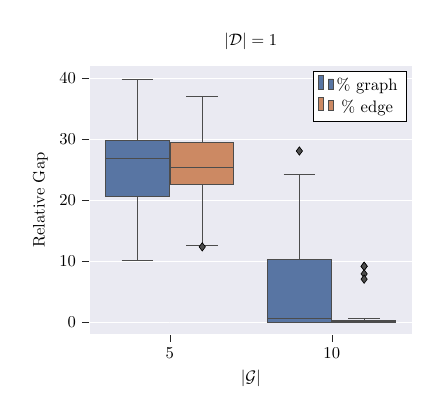
\begin{tikzpicture}[scale=0.6]

\begin{axis}[
axis background/.style={fill=color0},
axis line style={white},
tick align=outside,
title={$|\mathcal D| = 1$},
x grid style={white},
xtick pos = left,
ytick pos = left,
xlabel={$|\mathcal G|$},
xmin=-0.5, xmax=1.5,
xtick style={color=white!15!black},
xtick={0,1},
xticklabels={5,10},
y grid style={white},
ylabel={Relative Gap},
ymajorgrids,
ymin=-2.0023571013993, ymax=42.0494991293852,
ytick style={color=white!15!black}
]
\path [draw=white!29.8039215686275!black, fill=color1, semithick]
(axis cs:-0.396,20.6407800235787)
--(axis cs:-0.004,20.6407800235787)
--(axis cs:-0.004,29.8403354243381)
--(axis cs:-0.396,29.8403354243381)
--(axis cs:-0.396,20.6407800235787)
--cycle;
\path [draw=white!29.8039215686275!black, fill=color2, semithick]
(axis cs:0.004,22.6632155088597)
--(axis cs:0.396,22.6632155088597)
--(axis cs:0.396,29.3936680794107)
--(axis cs:0.004,29.3936680794107)
--(axis cs:0.004,22.6632155088597)
--cycle;
\path [draw=white!29.8039215686275!black, fill=color1, semithick]
(axis cs:0.604,0.0339850633863935)
--(axis cs:0.996,0.0339850633863935)
--(axis cs:0.996,10.2949188269681)
--(axis cs:0.604,10.2949188269681)
--(axis cs:0.604,0.0339850633863935)
--cycle;
\path [draw=white!29.8039215686275!black, fill=color2, semithick]
(axis cs:1.004,0.0194795130371425)
--(axis cs:1.396,0.0194795130371425)
--(axis cs:1.396,0.306707139438365)
--(axis cs:1.004,0.306707139438365)
--(axis cs:1.004,0.0194795130371425)
--cycle;
\draw[draw=white!29.8039215686275!black,fill=color1,line width=0.3pt] (axis cs:0,0) rectangle (axis cs:0,0);
\addlegendimage{ybar,ybar legend,draw=white!29.8039215686275!black,fill=color1,line width=0.3pt}
\addlegendentry{\% graph}

\draw[draw=white!29.8039215686275!black,fill=color2,line width=0.3pt] (axis cs:0,0) rectangle (axis cs:0,0);
\addlegendimage{ybar,ybar legend,draw=white!29.8039215686275!black,fill=color2,line width=0.3pt}
\addlegendentry{\% edge}

\addplot [semithick, white!29.8039215686275!black]
table {%
-0.2 20.6407800235787
-0.2 10.2174215472121
};
\addplot [semithick, white!29.8039215686275!black]
table {%
-0.2 29.8403354243381
-0.2 39.8372111596839
};
\addplot [semithick, white!29.8039215686275!black]
table {%
-0.298 10.2174215472121
-0.102 10.2174215472121
};
\addplot [semithick, white!29.8039215686275!black]
table {%
-0.298 39.8372111596839
-0.102 39.8372111596839
};
\addplot [semithick, white!29.8039215686275!black]
table {%
0.2 22.6632155088597
0.2 12.5823686637236
};
\addplot [semithick, white!29.8039215686275!black]
table {%
0.2 29.3936680794107
0.2 37.0654745861762
};
\addplot [semithick, white!29.8039215686275!black]
table {%
0.102 12.5823686637236
0.298 12.5823686637236
};
\addplot [semithick, white!29.8039215686275!black]
table {%
0.102 37.0654745861762
0.298 37.0654745861762
};
\addplot [black, mark=diamond*, mark size=2.5, mark options={solid,fill=white!29.8039215686275!black}, only marks]
table {%
0.2 12.3764537954977
};
\addplot [semithick, white!29.8039215686275!black]
table {%
0.8 0.0339850633863935
0.8 0
};
\addplot [semithick, white!29.8039215686275!black]
table {%
0.8 10.2949188269681
0.8 24.2898819355359
};
\addplot [semithick, white!29.8039215686275!black]
table {%
0.702 0
0.898 0
};
\addplot [semithick, white!29.8039215686275!black]
table {%
0.702 24.2898819355359
0.898 24.2898819355359
};
\addplot [black, mark=diamond*, mark size=2.5, mark options={solid,fill=white!29.8039215686275!black}, only marks]
table {%
0.8 28.0687173355187
};
\addplot [semithick, white!29.8039215686275!black]
table {%
1.2 0.0194795130371425
1.2 0
};
\addplot [semithick, white!29.8039215686275!black]
table {%
1.2 0.306707139438365
1.2 0.630772135488852
};
\addplot [semithick, white!29.8039215686275!black]
table {%
1.102 0
1.298 0
};
\addplot [semithick, white!29.8039215686275!black]
table {%
1.102 0.630772135488852
1.298 0.630772135488852
};
\addplot [black, mark=diamond*, mark size=2.5, mark options={solid,fill=white!29.8039215686275!black}, only marks]
table {%
1.2 7.94455506693244
1.2 9.18410909127298
1.2 9.19193054556677
1.2 7.08340072268779
};
\addplot [semithick, white!29.8039215686275!black]
table {%
-0.396 26.8781875312972
-0.004 26.8781875312972
};
\addplot [semithick, white!29.8039215686275!black]
table {%
0.004 25.341101423165
0.396 25.341101423165
};
\addplot [semithick, white!29.8039215686275!black]
table {%
0.604 0.591842201335821
0.996 0.591842201335821
};
\addplot [semithick, white!29.8039215686275!black]
table {%
1.004 0.0939379065004709
1.396 0.0939379065004709
};
\end{axis}
\end{tikzpicture}
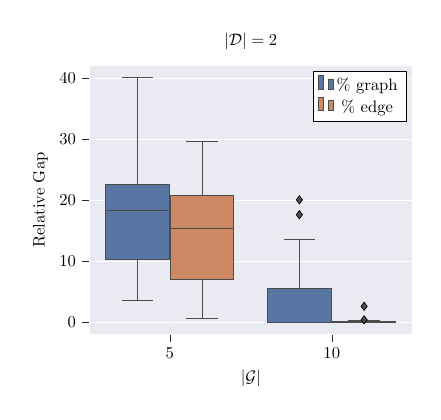
\begin{tikzpicture}[scale = 0.6]
\begin{axis}[
axis background/.style={fill=color0},
axis line style={white},
scaled y ticks=manual:{}{\pgfmathparse{#1}},
tick align=outside,
title={$|\mathcal D| = 2$},
x grid style={white},
xtick pos = left,
ytick pos = left,
xlabel={$|\mathcal G|$},
xmin=-0.5, xmax=1.5,
xtick style={color=white!15!black},
xtick={0,1},
xticklabels={5,10},
ylabel={Relative Gap},
y grid style={white},
ymajorgrids,
ymin=-2.0023571013993, ymax=42.0494991293852,
ytick style={color=white!15!black}
]
\path [draw=white!29.8039215686275!black, fill=color1, semithick]
(axis cs:-0.396,10.2866453493961)
--(axis cs:-0.004,10.2866453493961)
--(axis cs:-0.004,22.5081525206015)
--(axis cs:-0.396,22.5081525206015)
--(axis cs:-0.396,10.2866453493961)
--cycle;
\path [draw=white!29.8039215686275!black, fill=color2, semithick]
(axis cs:0.004,7.0678376200125)
--(axis cs:0.396,7.0678376200125)
--(axis cs:0.396,20.7415594727762)
--(axis cs:0.004,20.7415594727762)
--(axis cs:0.004,7.0678376200125)
--cycle;
\path [draw=white!29.8039215686275!black, fill=color1, semithick]
(axis cs:0.604,0)
--(axis cs:0.996,0)
--(axis cs:0.996,5.60272249505483)
--(axis cs:0.604,5.60272249505483)
--(axis cs:0.604,0)
--cycle;
\path [draw=white!29.8039215686275!black, fill=color2, semithick]
(axis cs:1.004,8.79818728320465e-05)
--(axis cs:1.396,8.79818728320465e-05)
--(axis cs:1.396,0.13797377094944)
--(axis cs:1.004,0.13797377094944)
--(axis cs:1.004,8.79818728320465e-05)
--cycle;
\draw[draw=white!29.8039215686275!black,fill=color1,line width=0.3pt] (axis cs:0,0) rectangle (axis cs:0,0);
\addlegendimage{ybar,ybar legend,draw=white!29.8039215686275!black,fill=color1,line width=0.3pt}
\addlegendentry{\% graph}

\draw[draw=white!29.8039215686275!black,fill=color2,line width=0.3pt] (axis cs:0,0) rectangle (axis cs:0,0);
\addlegendimage{ybar,ybar legend,draw=white!29.8039215686275!black,fill=color2,line width=0.3pt}
\addlegendentry{\% edge}
\draw[draw=white!29.8039215686275!black,fill=color1,line width=0.3pt] (axis cs:0,0) rectangle (axis cs:0,0);
\draw[draw=white!29.8039215686275!black,fill=color2,line width=0.3pt] (axis cs:0,0) rectangle (axis cs:0,0);
\addplot [semithick, white!29.8039215686275!black]
table {%
-0.2 10.2866453493961
-0.2 3.60268280881678
};
\addplot [semithick, white!29.8039215686275!black]
table {%
-0.2 22.5081525206015
-0.2 40.0471420279859
};
\addplot [semithick, white!29.8039215686275!black]
table {%
-0.298 3.60268280881678
-0.102 3.60268280881678
};
\addplot [semithick, white!29.8039215686275!black]
table {%
-0.298 40.0471420279859
-0.102 40.0471420279859
};
\addplot [semithick, white!29.8039215686275!black]
table {%
0.2 7.0678376200125
0.2 0.642284767544519
};
\addplot [semithick, white!29.8039215686275!black]
table {%
0.2 20.7415594727762
0.2 29.5674840057024
};
\addplot [semithick, white!29.8039215686275!black]
table {%
0.102 0.642284767544519
0.298 0.642284767544519
};
\addplot [semithick, white!29.8039215686275!black]
table {%
0.102 29.5674840057024
0.298 29.5674840057024
};
\addplot [semithick, white!29.8039215686275!black]
table {%
0.8 0
0.8 0
};
\addplot [semithick, white!29.8039215686275!black]
table {%
0.8 5.60272249505483
0.8 13.5020703882813
};
\addplot [semithick, white!29.8039215686275!black]
table {%
0.702 0
0.898 0
};
\addplot [semithick, white!29.8039215686275!black]
table {%
0.702 13.5020703882813
0.898 13.5020703882813
};
\addplot [black, mark=diamond*, mark size=2.5, mark options={solid,fill=white!29.8039215686275!black}, only marks]
table {%
0.8 20.0779538400286
0.8 17.6366857723062
};
\addplot [semithick, white!29.8039215686275!black]
table {%
1.2 8.79818728320465e-05
1.2 0
};
\addplot [semithick, white!29.8039215686275!black]
table {%
1.2 0.13797377094944
1.2 0.235568383869461
};
\addplot [semithick, white!29.8039215686275!black]
table {%
1.102 0
1.298 0
};
\addplot [semithick, white!29.8039215686275!black]
table {%
1.102 0.235568383869461
1.298 0.235568383869461
};
\addplot [black, mark=diamond*, mark size=2.5, mark options={solid,fill=white!29.8039215686275!black}, only marks]
table {%
1.2 2.63387588427892
1.2 0.424951172219
};
\addplot [semithick, white!29.8039215686275!black]
table {%
-0.396 18.3831443590176
-0.004 18.3831443590176
};
\addplot [semithick, white!29.8039215686275!black]
table {%
0.004 15.3701106859569
0.396 15.3701106859569
};
\addplot [semithick, white!29.8039215686275!black]
table {%
0.604 0.0593655722027036
0.996 0.0593655722027036
};
\addplot [semithick, white!29.8039215686275!black]
table {%
1.004 0.0126952901795616
1.396 0.0126952901795616
};
\end{axis}
\end{tikzpicture}
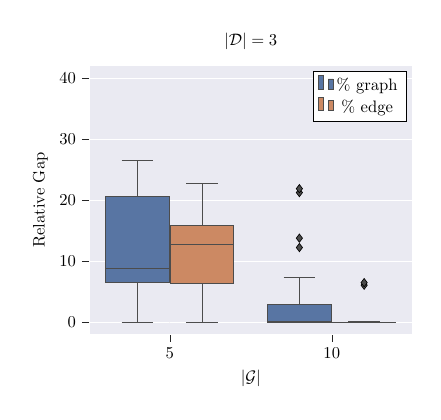
\begin{tikzpicture}[scale = 0.6]
\begin{axis}[
axis background/.style={fill=color0},
axis line style={white},
scaled y ticks=manual:{}{\pgfmathparse{#1}},
tick align=outside,
title={$|\mathcal D| = 3$},
x grid style={white},
xtick pos = left,
ytick pos = left,
xlabel={$|\mathcal G|$},
xmin=-0.5, xmax=1.5,
xtick style={color=white!15!black},
xtick={0,1},
xticklabels={5,10},
ylabel={Relative Gap},
y grid style={white},
ymajorgrids,
ymin=-2.0023571013993, ymax=42.0494991293852,
ytick style={color=white!15!black}
]
\path [draw=white!29.8039215686275!black, fill=color1, semithick]
(axis cs:-0.396,6.53463437293595)
--(axis cs:-0.004,6.53463437293595)
--(axis cs:-0.004,20.6227343985175)
--(axis cs:-0.396,20.6227343985175)
--(axis cs:-0.396,6.53463437293595)
--cycle;
\path [draw=white!29.8039215686275!black, fill=color2, semithick]
(axis cs:0.004,6.43445824030872)
--(axis cs:0.396,6.43445824030872)
--(axis cs:0.396,15.9075308578851)
--(axis cs:0.004,15.9075308578851)
--(axis cs:0.004,6.43445824030872)
--cycle;
\path [draw=white!29.8039215686275!black, fill=color1, semithick]
(axis cs:0.604,7.32352158495657e-08)
--(axis cs:0.996,7.32352158495657e-08)
--(axis cs:0.996,2.99868227559093)
--(axis cs:0.604,2.99868227559093)
--(axis cs:0.604,7.32352158495657e-08)
--cycle;
\path [draw=white!29.8039215686275!black, fill=color2, semithick]
(axis cs:1.004,0)
--(axis cs:1.396,0)
--(axis cs:1.396,0.0559914040218077)
--(axis cs:1.004,0.0559914040218077)
--(axis cs:1.004,0)
--cycle;
\draw[draw=white!29.8039215686275!black,fill=color1,line width=0.3pt] (axis cs:0,0) rectangle (axis cs:0,0);
\addlegendimage{ybar,ybar legend,draw=white!29.8039215686275!black,fill=color1,line width=0.3pt}
\addlegendentry{\% graph}

\draw[draw=white!29.8039215686275!black,fill=color2,line width=0.3pt] (axis cs:0,0) rectangle (axis cs:0,0);
\addlegendimage{ybar,ybar legend,draw=white!29.8039215686275!black,fill=color2,line width=0.3pt}
\addlegendentry{\% edge}
\draw[draw=white!29.8039215686275!black,fill=color1,line width=0.3pt] (axis cs:0,0) rectangle (axis cs:0,0);
\draw[draw=white!29.8039215686275!black,fill=color2,line width=0.3pt] (axis cs:0,0) rectangle (axis cs:0,0);
\addplot [semithick, white!29.8039215686275!black]
table {%
-0.2 6.53463437293595
-0.2 1.79056825828256e-05
};
\addplot [semithick, white!29.8039215686275!black]
table {%
-0.2 20.6227343985175
-0.2 26.5456799908282
};
\addplot [semithick, white!29.8039215686275!black]
table {%
-0.298 1.79056825828256e-05
-0.102 1.79056825828256e-05
};
\addplot [semithick, white!29.8039215686275!black]
table {%
-0.298 26.5456799908282
-0.102 26.5456799908282
};
\addplot [semithick, white!29.8039215686275!black]
table {%
0.2 6.43445824030872
0.2 0.0394119649305478
};
\addplot [semithick, white!29.8039215686275!black]
table {%
0.2 15.9075308578851
0.2 22.8058892464428
};
\addplot [semithick, white!29.8039215686275!black]
table {%
0.102 0.0394119649305478
0.298 0.0394119649305478
};
\addplot [semithick, white!29.8039215686275!black]
table {%
0.102 22.8058892464428
0.298 22.8058892464428
};
\addplot [semithick, white!29.8039215686275!black]
table {%
0.8 7.32352158495657e-08
0.8 0
};
\addplot [semithick, white!29.8039215686275!black]
table {%
0.8 2.99868227559093
0.8 7.36554173175818
};
\addplot [semithick, white!29.8039215686275!black]
table {%
0.702 0
0.898 0
};
\addplot [semithick, white!29.8039215686275!black]
table {%
0.702 7.36554173175818
0.898 7.36554173175818
};
\addplot [black, mark=diamond*, mark size=2.5, mark options={solid,fill=white!29.8039215686275!black}, only marks]
table {%
0.8 12.2593696921256
0.8 21.2612364965465
0.8 21.8997819287943
0.8 13.7961652594506
};
\addplot [semithick, white!29.8039215686275!black]
table {%
1.2 0
1.2 0
};
\addplot [semithick, white!29.8039215686275!black]
table {%
1.2 0.0559914040218077
1.2 0.109590853639457
};
\addplot [semithick, white!29.8039215686275!black]
table {%
1.102 0
1.298 0
};
\addplot [semithick, white!29.8039215686275!black]
table {%
1.102 0.109590853639457
1.298 0.109590853639457
};
\addplot [black, mark=diamond*, mark size=2.5, mark options={solid,fill=white!29.8039215686275!black}, only marks]
table {%
1.2 6.08934722229896
1.2 6.51363062749102
};
\addplot [semithick, white!29.8039215686275!black]
table {%
-0.396 8.85165952119232
-0.004 8.85165952119232
};
\addplot [semithick, white!29.8039215686275!black]
table {%
0.004 12.7294513588976
0.396 12.7294513588976
};
\addplot [semithick, white!29.8039215686275!black]
table {%
0.604 0.0906636339713724
0.996 0.0906636339713724
};
\addplot [semithick, white!29.8039215686275!black]
table {%
1.004 0.00552917704183977
1.396 0.00552917704183977
};
\end{axis}
\end{tikzpicture}
\caption{Relative gap boxplots}
\label{fig:gap_boxplot}
\end{figure}
\noindent
The boxplots in Figure \ref{fig:gap_boxplot} represent the relative gap of the solution provided by the matheuristic with respect to the one provided by the exact solution of the mathematical programming model within the time limit, with the initialization of the solution found by the matheuristic.\LA{ We can observe that the maximum value of the relative gap is equal to 40, but it decreases when the number of target graphs increases from 5 to 10 and it tends to be smaller when a given fraction of each edge must be visited with respect to the other case, that is, when a given fraction of each graph to be visited is imposed. In particular, for the instances with 10 target graphs, the relative gap is not greater than 25, with the exception of one outlier in the case with 1 drone and a given fraction of each graph to be visited. When the number of drones is equal to 2, this maximum value further decreases and it becomes lower than 10 when the fleet consists of 3 drones. Additionally, when a given fraction of each edge to be visited is imposed, the relative gap is even smaller and around zero in most of the instances. Thus, we can conclude that the matheuristic, even if it does not speed up the convergence to the optimum, it provides solutions of good quality, especially for instances of large size, both in terms of target graphs and drones, and for the most challenging variant of the problem in which a given fraction of each edge must be visited.}
